
%(BEGIN_QUESTION)
% Copyright 2012, Tony R. Kuphaldt, released under the Creative Commons Attribution License (v 1.0)
% This means you may do almost anything with this work of mine, so long as you give me proper credit

In this process, steam heat is supposed to maintain the temperature of solvent in the tank at 105 $^{o}$F:

$$\includegraphics[width=15.5cm]{i0006rx01.eps}$$

Suppose the steam pressure indicated by PG-365 is 30 PSIG, and we know that this steam is saturated (i.e. it's right at the boiling/condensing temperature for that pressure).  Condensate (water) exits the heating loop at 145 $^{o}$F as indicated by TG-205.  PG-361 shows the condensate line to be at atmospheric pressure (0 PSIG).

Assuming a steam flow rate of 15 pounds per hour, calculate the approximate amount of time required to heat a new batch of solvent from ambient temperature (50 $^{o}$F) up to 105 $^{o}$F, if the stored volume of solvent is 4300 gallons, and the solvent happens to have a density of 57 lb/ft$^{3}$ and a specific heat of 0.73.  Feel free to neglect details such as heat loss through the insulation of the tank wall, and simply treat this as a heat input / temperature rise thermodynamics problem.

\underbar{file i00973}
%(END_QUESTION)





%(BEGIN_ANSWER)

I won't reveal the solution in its entirety here, but this problem essentially breaks down into a few simple parts:

\begin{itemize}
\item{} Figuring out how much heat will be required to raise the solvent's temperature
\item{} Figuing out how fast heat is delivered by the steam at the given mass flow rate
\item{} Dividing \underbar{required heat} (BTU) by \underbar{heat rate} (BTU/hr) to solve for \underbar{time} (hr)
\end{itemize}

Determining heat rate delivered by the steam is most easily done using a {\it steam table}.

%(END_ANSWER)





%(BEGIN_NOTES)

First, let's calculate the amount of heat needed to do the job of warming all that solvent from 50 $^{o}$F to 105 $^{o}$F.  We know that this will be a specific heat problem, and therefore we will need to know the total {\it mass} of 4300 gallons of this solvent:

$$\left( {4300 \hbox{ gal} \over 1} \right)  \left({231 \hbox{ in}^3 \over 1 \hbox{ gal}} \right) \left( {1 \hbox{ ft}^3 \over 1728 \hbox{ in}^3} \right)  \left( {57 \hbox{ lb} \over \hbox{ft}^3} \right) = 32765.1 \hbox{ lb}$$

Now that we know the solvent's mass, we may calculate for required heat:

$$Q = mc \Delta T$$
 
$$Q = (32765.1 \hbox{ lb}) (0.73 \hbox{ BTU/lb}\cdot^o\hbox{F}) (105^o \hbox{F} - 50^o \hbox{F}) $$

$$Q = 1315518.9 \hbox{ BTU}$$

If we calculate how much heat is transferred per pound of saturated steam to the solvent, we may then calculate the {\it rate} of heat transfer knowing the flow of steam is 15 pounds per hour.  The calculation of heat liberated by the steam is a matter of subtracting {\it enthalpy} figures for the steam and for the condensate:

\vskip 10pt

Enthalpy of 30 PSI saturated steam (from steam table) = 1171.5 BTU per pound 

\vskip 10pt

Enthalpy of 145 $^{o}$F condensate = 113 BTU per pound 

\vskip 10pt

Heat lost by condensing steam = 1171.5 $-$ 113 = 1058.5 BTU per pound

\vskip 10pt

At a flow rate of 15 pounds per hour, this equates to a heat transfer rate of 15877.5 BTU per hour.  This is the rate at which thermal energy is being delivered to the solvent tank by the steam.

\vskip 10pt

Dividing this heat rate figure into the total heat needed (1315518.9 BTU) yields a heating time of {\bf 82.85 hours}.

\vskip 10pt

Some important factors have been omitted from this calculation, including heat loss through the insulation of the storage tank, and throttling of control valve TCV-105 as the solvent approaches setpoint temperature.  Both factors will work to {\it lengthen} the amount of time required to bring the solvent up to its final temperature of 105 $^{o}$F.

%INDEX% Physics, heat and temperature: saturated steam pressure versus temperature
%INDEX% Physics, heat and temperature: steam table
%INDEX% Process: solvent storage tank (realistic P&ID shown)

%(END_NOTES)


